\documentclass[11pt,a4paper]{article}
\usepackage[margin=1in]{geometry}
\usepackage{amsmath,amssymb}
\usepackage{graphicx}
\usepackage{booktabs}
\usepackage{hyperref}
\usepackage{xcolor}
\usepackage{caption}
\usepackage{subcaption}
\usepackage{enumitem}
\usepackage{parskip}
\usepackage{microtype}
\usepackage{float}
\usepackage{array}
\hypersetup{colorlinks=true, linkcolor=blue, citecolor=blue, urlcolor=blue}
\captionsetup{font=small,labelfont=bf}
\setlist{nosep}
\graphicspath{{figures/}}\emergencystretch=4em

\title{\textbf{AE646 --- Final Report (Stage 3)}\\[0.4em]
\large Optimising a Fourier Neural Operator for Parametric Darcy Flow:\\
Recipe, Architecture, Data, Resolution, Latency and Comparison with a Finite-Volume Solver}
\author{Team PINNacles\\Aryamann Srivastava, Varun Sathaye, Atishay Jain, Vedant S.\ Tiwari\\Department of Aerospace Engineering, IIT Kanpur}
\date{November 2026}

\begin{document}
\maketitle

\begin{abstract}
We study a Fourier Neural Operator (FNO) and an MLP baseline as surrogates for the 2D Darcy flow equation $-\nabla\!\cdot(\kappa\nabla u)=1$ on real PDEBench data (900/100/200 train/validation/test split, $64\times64$). Stage~2 reported FNO $0.052$ vs.\ MLP $0.082$ mean relative $L_2$ error. In Stage~3 we show that most of the remaining error was \emph{optimisation}, not capacity: replacing the Stage~2 recipe (MSE loss, a learning rate that restarted every 200 steps, no augmentation) by a relative-$L_2$ loss, a single cosine decay and dihedral-symmetry (D4) augmentation halves the FNO error at an identical 5\,700-step budget ($0.052\to0.025$; 3 seeds) and helps the MLP too ($0.080\to0.045$). Validation-only selection over modes, width, depth, steps and optimiser settings gives a final FNO (9.5\,M parameters) with test error $0.0202\pm0.0004$ (5 seeds) against $0.0415\pm0.0009$ for an equally tuned 100\,M-parameter MLP: the FNO advantage \emph{grows} from $1.6\times$ to $2.05\times$. The FNO error plateaus at $\approx0.02$ for $\ge 5{,}000$ training samples and is nearly insensitive to the number of Fourier modes ($\ge 4$). Against a properly implemented vectorised finite-volume solver, calibrated on validation data, the FNO is more accurate than the solver at the same resolution ($0.020$ vs.\ $0.044$ at $64\times64$) and $5$--$35\times$ faster on a GPU, but \emph{not} faster on a single CPU core. We correct the Stage~2 speed-up claim ($1443\times$ vs.\ 1030\,ms), which used an inefficient reference solver. Physical diagnostics (PDE residual, boundary values, positivity, error vs.\ interface distance and permeability composition) show that the residual error is concentrated in a few low-contrast/uniform-$\kappa$ fields with large pressure amplitude.
\end{abstract}

\section{Introduction and Scope}
The physical problem is steady single-phase flow in a heterogeneous porous medium: $-\nabla\!\cdot(\kappa\nabla u)=f$ on $(0,1)^2$ with $u=0$ on the boundary and $f=1$, where $\kappa\in\{0.1,1.0\}$ is a piecewise-constant permeability and $u$ the pressure. The SciML task is to learn the operator $\mathcal G:\kappa\mapsto u$. Baseline: an MLP; SciML model: FNO~\cite{li2021fno}; data: PDEBench 2D Darcy ($\beta=1$)~\cite{takamoto2022pdebench}.

Stage~2 delivered the pipeline, EDA, preprocessing/baseline ablations and a first MLP-vs-FNO comparison. Stage~3 asks: \emph{how good can the FNO be made, what limits it, what does it cost, and how does it compare with a classical solver?} We answer with five controlled studies (\S\ref{sec:recipe}--\S\ref{sec:solver}) and a physical analysis (\S\ref{sec:physics}). Every number below comes from a run whose configuration and metrics are stored in \texttt{results/stage3/}.

\section{Data, Protocol and Metric}
The split is unchanged from Stage~2 (seed 42): 900 train, 100 validation, 200 test samples out of 1\,200 drawn from the 10\,000 real PDEBench fields; inputs are $\kappa$ plus $(x,y)$ coordinate channels, standardised with training statistics; the $128\times128$ fields are stride-2 subsampled to $64\times64$ (\S\ref{sec:res} also uses 32 and 128). The other 8\,800 real samples were never used in Stage~1--2 and appear only in the data-scaling study. \textbf{All hyper-parameter and design choices are made on the validation set; the test set is evaluated once per run.} The metric is the per-sample relative $L_2$ error $\|\hat u-u\|_2/\|u\|_2$ in physical (de-normalised) units, averaged over test samples. Unless stated otherwise, ``$\pm$'' is the standard deviation over seeds.

\textbf{Symmetry.} The data are statistically invariant under the dihedral group D4 (rotations/reflections of the square), and the PDE with $f=1$ and homogeneous Dirichlet conditions is exactly equivariant. We therefore (i) augment training with a random D4 element per batch, applied at $128\times128$ \emph{before} sub-sampling (rotating an already sub-sampled field would shift the grid phase and is not valid), and (ii) optionally average predictions over the group at test time (TTA; at $64\times64$ only \{identity, transpose\} are phase-consistent, so TTA there is a 2-element average). The Stage~2 protocol (100 epochs $=$ 5\,700 steps, batch 16) is kept as the reference \emph{step budget}.

\section{Models}
\textbf{FNO2d}: lifting $3\to w$; $L$ Fourier layers, each combining a spectral convolution (rfft2, learned complex weights on the lowest $m\times m$ modes of two frequency bands, irfft2), a $1\times1$ convolution bypass, layer normalisation and GELU; projection $w\to128\to1$. Stage~2 configuration: $m=12$, $w=64$, $L=4$ (4.74\,M parameters). \textbf{MLP}: flatten $64^2\!\cdot\!3$, three hidden layers, GELU, output $64^2$ (Stage~2: $3\times2048$, 42\,M parameters). Both use AdamW.

\section{Study 1 --- What Limited Stage~2? The Training Recipe}\label{sec:recipe}
While designing Stage~3 we found two properties of the Stage~2 recipe: the loss was MSE on standardised pressure (whereas the reported metric is a \emph{relative} error, so low-amplitude samples were under-weighted), and the cosine schedule was stepped per batch with $T_{\max}$ equal to the number of epochs, so the learning rate cycled $10^{-3}\to0$ every 200 steps ($\approx$28 cycles) instead of decaying once. We reproduced this recipe exactly (row~1 of Table~\ref{tab:recipe}: $0.0524\pm0.0018$, matching the reported $0.052$) and ablated each change at the same 5\,700-step budget, three seeds each.

\begin{table}[H]\centering\small
\caption{Recipe ablation, 5\,700 steps, test relative $L_2$ (mean $\pm$ sd, 3 seeds). TTA = 2-element symmetrisation.}\label{tab:recipe}
\begin{tabular}{llllcc}\toprule
schedule & loss & aug. & FNO (4.7\,M) & FNO + TTA & MLP (42\,M)\\\midrule
restarting (Stage 2) & MSE & none & $0.0524\pm0.0018$ & 0.0482 & $0.0802\pm0.0031$\\
single cosine & MSE & none & $0.0485\pm0.0008$ & 0.0444 & $0.0719\pm0.0010$\\
restarting & rel-$L_2$ & none & $0.0389\pm0.0002$ & 0.0366 & $0.0630\pm0.0017$\\
restarting & MSE & D4 & $0.0451\pm0.0028$ & 0.0416 & $0.0817\pm0.0008$\\
single cosine & rel-$L_2$ & none & $0.0384\pm0.0004$ & 0.0359 & $0.0612\pm0.0008$\\
restarting & rel-$L_2$ & D4 & $0.0286\pm0.0001$ & 0.0266 & $0.0518\pm0.0010$\\
single cosine & MSE & D4 & $0.0369\pm0.0004$ & 0.0343 & $0.0649\pm0.0004$\\
\textbf{single cosine} & \textbf{rel-$L_2$} & \textbf{D4} & $\mathbf{0.0249\pm0.0002}$ & \textbf{0.0237} & $\mathbf{0.0454\pm0.0003}$\\\bottomrule
\end{tabular}\end{table}

\begin{figure}[H]\centering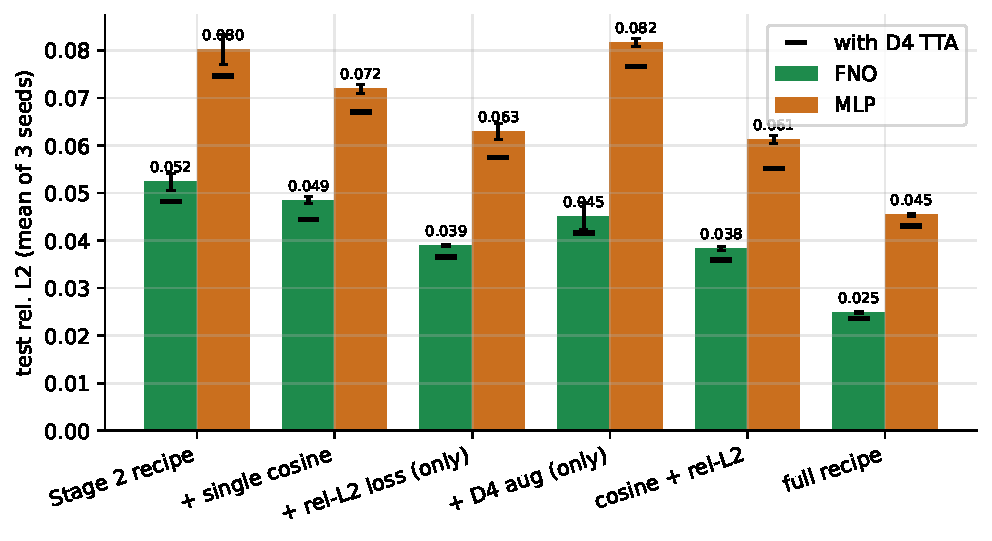
\includegraphics[width=0.8\linewidth]{fig_recipe_ablation.pdf}
\caption{Recipe ablation (bars: test error, error bars: sd over 3 seeds; black ticks: with TTA).}\label{fig:recipe}\end{figure}

The relative-$L_2$ loss is the largest single gain ($-26\%$ for the FNO), D4 augmentation adds a further $-35\%$ on top of it, and the schedule fix contributes $\approx-7\%$; the full recipe halves the FNO error and reduces the MLP error by $43\%$ at identical cost. D4 augmentation \emph{alone} does not help under the MSE loss and the restarting schedule (MLP: $0.0817$ vs.\ $0.0802$, within noise), so the gains are interactions: better-optimised training is what lets the model use the 8$\times$ larger effective data set. The FNO retains its advantage everywhere ($1.8\times$ better in the full recipe, vs.\ $1.5\times$ with the Stage~2 recipe). All later studies use the full recipe.

\section{Study 2 --- Optimising the FNO Architecture}\label{sec:arch}
With the full recipe and 20\,000 steps we varied one factor at a time around $(m,w,L)=(12,64,4)$, then trained joint candidates for 60\,000 steps (Figure~\ref{fig:arch}, Table~\ref{tab:arch}).

\begin{figure}[H]\centering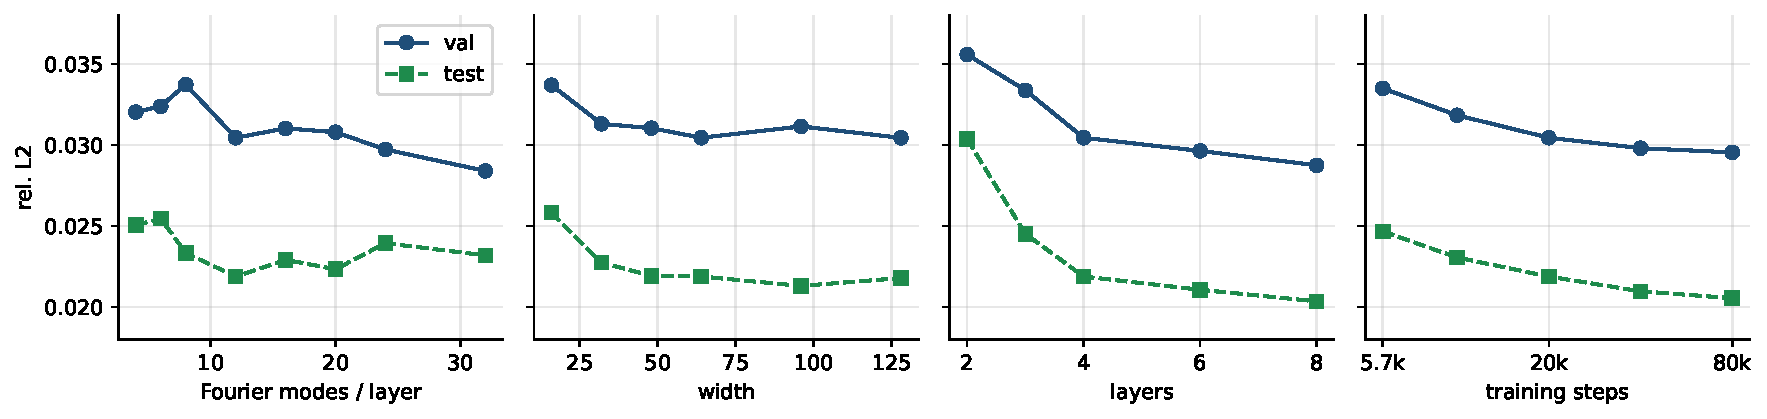
\includegraphics[width=\linewidth]{fig_arch_sweeps.pdf}
\caption{One-factor sweeps (single seed, full recipe, 20\,000 steps except the step sweep). Blue: validation, green: test. Seed-to-seed sd is $\approx0.0004$.}\label{fig:arch}\end{figure}

\begin{table}[H]\centering\small
\caption{Selection by validation error. Left: joint candidates, 60\,000 steps, one seed. Right: MLP capacity, 20\,000 steps.}\label{tab:arch}
\setlength{\tabcolsep}{4pt}\begin{tabular}{lcccc}\toprule
FNO $(m,w,L)$ & params & val & test & \\\midrule
(12, 64, 4) & 4.7\,M & 0.0298 & 0.0212 & \\
(16, 64, 6) & 12.6\,M & 0.0286 & 0.0210 & \\
(16, 96, 6) & 28.4\,M & 0.0281 & 0.0203 & \\
(16, 96, 8) & 37.8\,M & 0.0284 & 0.0198 & \\
\textbf{(12, 64, 8)} & \textbf{9.5\,M} & \textbf{0.0273} & 0.0200 & \textbf{selected}\\\bottomrule
\end{tabular}\hspace{0.8em}
\begin{tabular}{lccc}\toprule
MLP hidden & params & val & test\\\midrule
$2\times1024$ & 17.8\,M & 0.0513 & 0.0463\\
$3\times1024$ & 18.9\,M & 0.0469 & 0.0412\\
$3\times2048$ & 42.0\,M & 0.0477 & 0.0399\\
$5\times2048$ & 50.4\,M & 0.0509 & 0.0462\\
\textbf{$3\times4096$} & \textbf{100.7\,M} & \textbf{0.0461} & 0.0404\\\bottomrule
\end{tabular}\end{table}

\textbf{Findings.} (i) The FNO is remarkably insensitive to width ($\ge32$) and to the number of retained modes ($\ge 8$; the whole $m\in[4,32]$ range spans only $0.022$--$0.025$ test error, while parameters grow from 0.5\,M to 33.6\,M). (ii) Depth and training length help slowly: $L=2\to8$ gives $0.030\to0.020$; 5\,700$\to$80\,000 steps gives $0.0247\to0.0205$. (iii) Learning rate ($5\!\times\!10^{-4}$--$2\!\times\!10^{-3}$), weight decay ($0$--$10^{-2}$) and batch size (8--32) change the test error by $<0.001$. (iv) The best validation error selects a deeper, \emph{not wider} model, $(12,64,8)$; larger models are not better on validation. The differences among the top candidates are of the order of the seed noise, so we chose the smallest model within it. The MLP was tuned on the same footing; its validation-best is $3\times4096$ (100\,M parameters), and larger MLPs do not fix its gap. \emph{Final models} were retrained with 5 seeds for 60\,000 steps:

\begin{table}[H]\centering\small
\caption{Final models (60\,000 steps, full recipe, 5 seeds, test set of 200 fields).}\label{tab:final}
\begin{tabular}{lcccc}\toprule
model & params & mean rel.\ $L_2$ & median & with 2-elem.\ TTA\\\midrule
Stage 2 FNO (reported) & 4.7\,M & 0.0521 & 0.0398 & --\\
Stage 2 MLP (reported) & 42.0\,M & 0.0820 & 0.0695 & --\\
\textbf{Final FNO} & 9.5\,M & $\mathbf{0.0202\pm0.0004}$ & 0.0070 & $0.0200\pm0.0003$\\
\textbf{Final MLP} & 100.7\,M & $0.0415\pm0.0009$ & 0.0272 & $0.0386\pm0.0009$\\\bottomrule
\end{tabular}\end{table}
Training the final FNO takes $\approx32$\,min on one shared GPU. The FNO error is 2.6$\times$ lower than the Stage~2 FNO and 2.05$\times$ lower than the best MLP, with 10.6$\times$ fewer parameters. The median FNO error is only $0.7\%$: the mean is dominated by a small tail (\S\ref{sec:physics}).

\section{Study 3 --- Data Scaling and Resolution}\label{sec:res}
\textbf{Data scaling.} We trained FNO $(12,64,4)$ and the $3\times2048$ MLP with $n\in\{100,\dots,9700\}$ samples (900 course samples plus the unused real data; fixed 20\,000 steps, 2 seeds each, TTA).

\begin{figure}[H]\centering
\begin{subfigure}{0.49\linewidth}\centering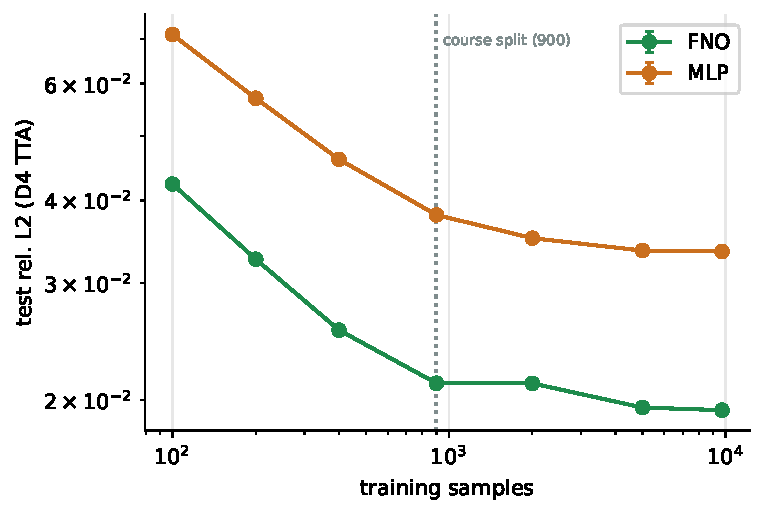
\includegraphics[width=\linewidth]{fig_data_scaling.pdf}\caption{Data scaling}\end{subfigure}
\begin{subfigure}{0.40\linewidth}\centering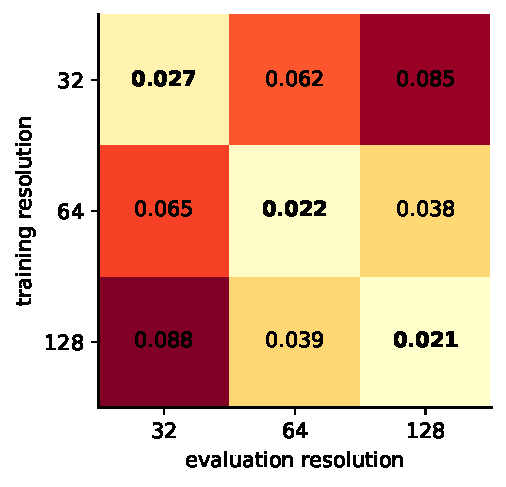
\includegraphics[width=\linewidth]{fig_resolution.pdf}\caption{Train vs.\ evaluation resolution}\end{subfigure}
\caption{(a) FNO error falls from $0.042$ ($n=100$) to $0.0195$ ($n=5000$) and then saturates; at 200 samples the FNO is at $0.033$ vs.\ $0.057$ for the MLP, which plateaus at $0.034$. (b) Test error of FNOs trained at one resolution and evaluated at another (2 seeds).}\label{fig:scaling}\end{figure}

The FNO is much more sample-efficient: with 400 samples it is already better than the MLP with 9\,700, and at $n=900$ the ratio is $1.8\times$. The FNO plateau at $\approx0.019$--$0.020$ for $n\ge5000$ cannot be broken by more data at this resolution and model size, which points to a resolution/representation floor rather than a data floor (see \S\ref{sec:physics}).

\textbf{Resolution.} FNOs trained at 32, 64 and 128 and evaluated at all three resolutions (Fig.~\ref{fig:scaling}b). In-resolution errors are $0.027$, $0.022$, $0.021$: refining from 64 to 128 gains only $\approx4\%$ while costing $4\times$ more compute. Zero-shot transfer works but is far from free: a model trained at 64 attains $0.038$ at 128 (the final 60\,000-step model: $0.037$) and $0.065$ at 32 (final: $0.063$), i.e.\ 1.7--3$\times$ worse than a native-resolution model; coarse-trained models transfer worst ($0.085$ at 128). Zero-shot super-resolution is therefore useful for cheap grid refinement, but ``resolution-independent'' should be read as \emph{applicable} at any resolution, not \emph{accurate} at any resolution: the input statistics and discretisation error of the target change with the grid.

\section{Study 4 --- Comparison with a Finite-Volume Solver and Inference Cost}\label{sec:solver}
\textbf{A correction.} Stage~2 reported FNO speed-ups of $1443\times$ and $7740\times$ relative to a 1030\,ms FDM solve. That reference used a solver whose boundary rows were set in a Python loop over sparse-matrix rows, which is orders of magnitude slower than a competent implementation; \emph{those speed-up figures are withdrawn}. We wrote a vectorised cell-centred finite-volume solver (\texttt{src/solvers.py}: COO assembly, sparse LU, and algebraic-multigrid-preconditioned CG via \texttt{pyamg}); the two solvers agree to $10^{-9}$.

\textbf{Which discretisation reproduces the ground truth?} Ideal cell-centred FV (Dirichlet boundary half a cell outside the array) differs from PDEBench's arrays by 5--10\%, because the reference data behave as if the Dirichlet boundary were about one cell outside the grid. We therefore calibrated the face averaging and boundary distance $b$ per resolution on 40 validation fields (Table~\ref{tab:solver}), i.e.\ we give the classical solver the same advantage of tuning to the data that the FNO gets by training on it. Coarse grids use stride sub-sampling of both $\kappa$ and $u$, exactly as the FNO sees them.

\begin{table}[H]\centering\small
\caption{FV solver vs.\ ground truth (test set) and cost (median of 40 solves, 1 CPU thread).}\label{tab:solver}
\begin{tabular}{lccccc}\toprule
grid & calibration & err.\ strict FV & err.\ calibrated & direct LU [ms] & AMG-CG [ms]\\\midrule
$32\times32$ & harmonic, $b{=}0.7$ & 0.098 & 0.094 & 1.8 & 5.5\\
$64\times64$ & harmonic, $b{=}0.8$ & 0.059 & 0.044 & 7.1 & 11.6\\
$128\times128$ & arithmetic, $b{=}1.05$ & 0.051 & 0.024 & 37.4 & 30.7\\\bottomrule
\end{tabular}\end{table}

\textbf{Latency.} We timed the final models with CUDA events on an idle RTX PRO 6000 (Blackwell) GPU and with wall-clock on the CPU of the shared 16-core host (CPU numbers are indicative only).

\begin{table}[H]\centering\small
\caption{Inference time per solution at $64\times64$ (median over repetitions). b = batch size, smp = sample; GPU batch-1 latency is kernel-launch bound.}\label{tab:lat}
\begin{tabular}{lcccc}\toprule
& test err. & GPU, b=1 [ms] & GPU, b=128 [ms/smp] & CPU8, b=32 [ms/smp]\\\midrule
Final FNO (9.5\,M) & 0.0202 & 1.44 & 0.20 & 16.5\\
FNO 4-layer (4.7\,M) & 0.0212 & 0.79 & 0.106 & --\\
Final MLP (100.7\,M) & 0.0415 & 0.27 & 0.0058 & 0.57\\
FV solver, $N{=}64$ & 0.044 & \multicolumn{3}{l}{7.1 ms (1 CPU thread)}\\
FV solver, $N{=}128$ & 0.024 & \multicolumn{3}{l}{37.4 ms (1 CPU thread)}\\\bottomrule
\end{tabular}\end{table}

\begin{figure}[H]\centering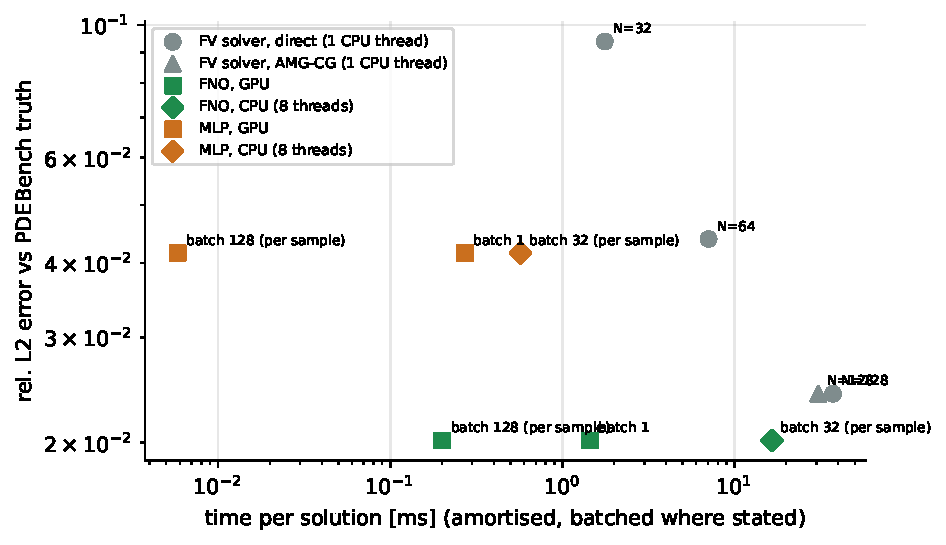
\includegraphics[width=0.72\linewidth]{fig_pareto.pdf}
\caption{Error--time trade-off. Solver: 1 CPU thread. FNO/MLP: GPU or 8-thread CPU as marked.}\label{fig:pareto}\end{figure}

\textbf{Reading the comparison.} (i) At the same $64\times64$ resolution the FNO agrees with the ground truth $2.2\times$ better than the calibrated solver ($0.020$ vs.\ $0.044$) and is $5\times$ (batch 1) to $35\times$ (batched) faster on a GPU; it is even more accurate than the $128\times128$ solver (0.024) while $26$--$187\times$ faster. (ii) The FNO's advantage in \emph{agreement with the data} is partly because it learns the data-generator's own discretisation quirks (the effective boundary offset) that a standard FV scheme does not share; it is a statement about this dataset, not a claim of higher fidelity to the continuous PDE. (iii) On one CPU core the FNO is \emph{not} faster: 37\,ms at batch 1, versus 7\,ms for the $64^2$ solver. The surrogate pays off through GPU batching and amortisation: training costs $\approx32$\,min ($\approx1.9\times10^3$\,s), so it breaks even with the $128^2$ solver after $\approx5\times10^4$ solves on one core. (iv) The MLP is the fastest model (0.006\,ms/sample) but $2\times$ less accurate than the FNO. (v) TF32 does not accelerate the FNO ($1.47$ vs.\ $1.44$\,ms), and \texttt{bfloat16} autocast is unsupported by PyTorch for the complex FFT operations, so mixed precision is not an easy lever here.

\section{Physical Interpretation}\label{sec:physics}
All diagnostics use the seed-0 final FNO on the 200 test fields (\texttt{src/stage3\_diagnostics.py}).

\begin{figure}[H]\centering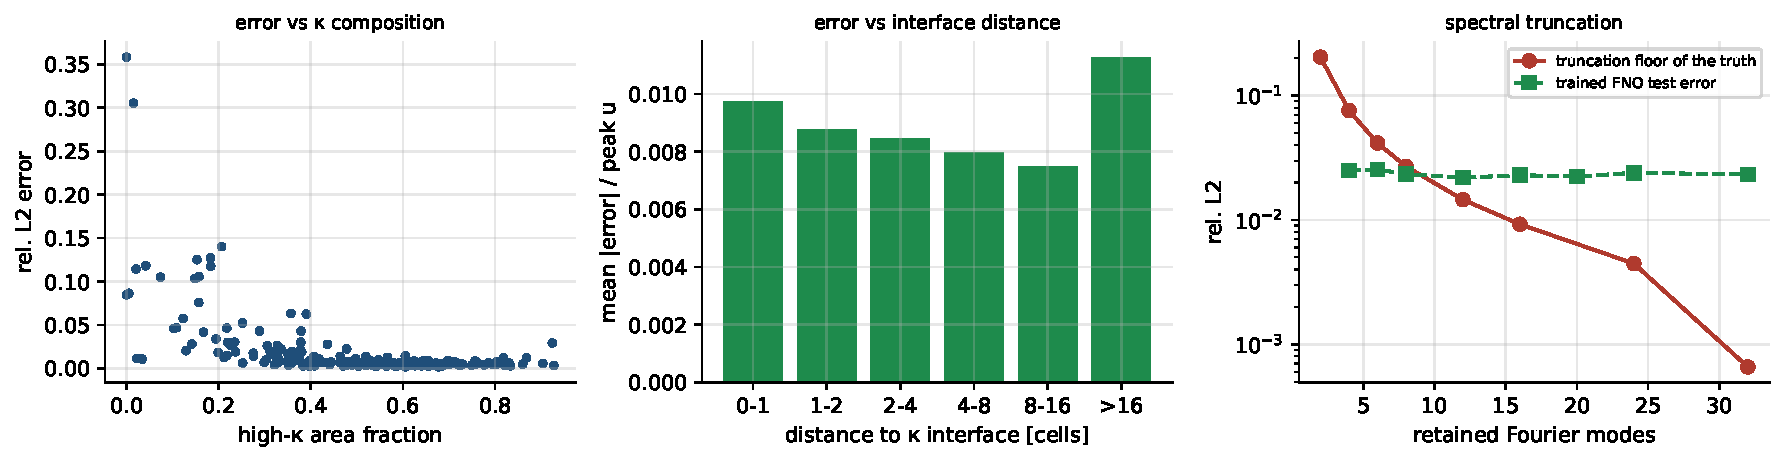
\includegraphics[width=\linewidth]{fig_diagnostics.pdf}
\caption{Left: error vs.\ high-permeability area fraction. Middle: mean absolute error (relative to the field's peak pressure) vs.\ distance to the nearest $\kappa$ interface. Right: relative error of the truth when truncated to $m$ Fourier modes (red) vs.\ the test error of FNOs actually trained with $m$ modes (green).}\label{fig:diag}\end{figure}

\textbf{Where the error is.} The median error is $0.7\%$ but the mean is $2.0\%$: the two exactly uniform-$\kappa$ test fields have errors $0.36$ and $0.085$, and excluding them the mean falls to $1.8\%$; the 90th percentile is $4.6\%$. Errors correlate with the peak pressure ($r=0.61$) and negatively with the high-$\kappa$ area fraction ($r=-0.55$): low-permeability-dominated fields have the largest pressure amplitudes because $u\propto1/\kappa$, and a network that must infer the overall amplitude from a near-constant input has the least information about it (Figure~\ref{fig:samples}, bottom row: correct shape, wrong amplitude). Contrary to the common expectation that neural surrogates fail at material interfaces, the error is only mildly larger at interfaces (0.0098 in the 0--1 cell band) than 8--16 cells away (0.0075), and largest in the interior of large regions (0.0112 beyond 16 cells), i.e.\ where the pressure peaks.

\textbf{Does the prediction obey the physics?} The relative residual of the finite-volume operator applied to the FNO prediction is $4.25$, versus $4.01$ for the ground truth itself: the residual is large in both because the truth is only a second-order accurate solution on the sub-sampled grid, but the FNO prediction is within $6\%$ of the truth's own residual, so it satisfies the discrete equation as well as the reference does at this resolution. The mean of the pressure field (an integral flux-balance quantity) is reproduced to $1.7\%$; only $1.5\times10^{-5}$ of the predicted pixels are negative (the maximum principle requires $u\ge0$); and the mean value on the outermost pixel ring relative to the interior is $0.1157$ (truth: $0.1159$), so the Dirichlet behaviour is learned rather than imposed.

\textbf{Spectral view.} The truth truncated to $m=4/8/12/16$ modes has relative error $7.6/2.7/1.5/0.9\%$, so at least $\approx12$ modes are needed to represent the solution linearly in Fourier space. Yet an FNO trained with only 4 modes reaches $2.5\%$: the spectral weights are not a hard band limit, because the $1\times1$ bypass, the pointwise nonlinearities and depth regenerate high-frequency content. Beyond $\approx8$ modes the accuracy is insensitive to $m$ (Fig.~\ref{fig:diag}, right), and so the observed $\approx0.02$ plateau is set by the amplitude/generalisation problem above and the input discretisation, not by the number of modes.

\begin{figure}[H]\centering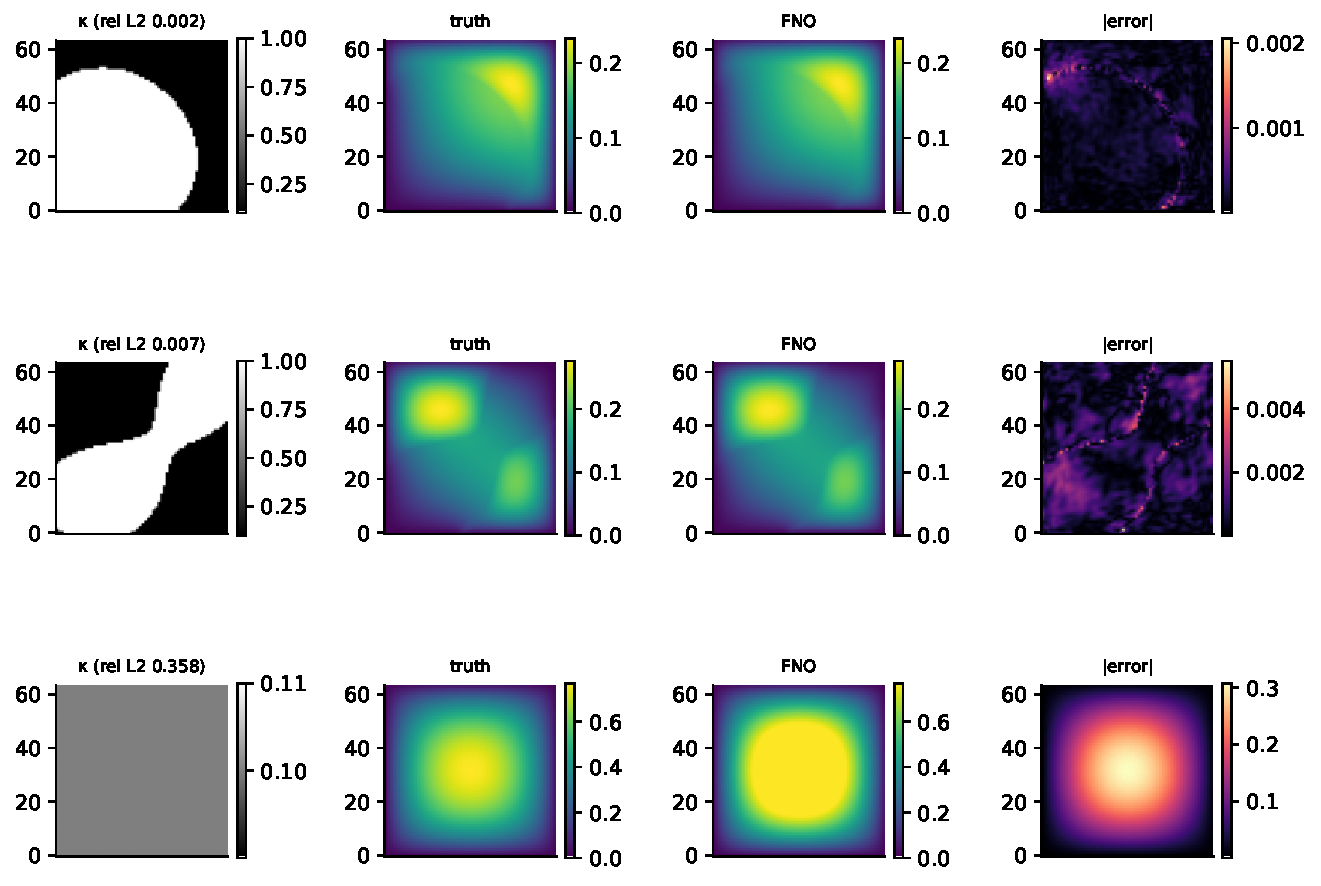
\includegraphics[width=0.66\linewidth]{fig_samples.pdf}
\caption{Best, median and worst test sample of the final FNO: $\kappa$ (relative error in title), truth, prediction, absolute error. The worst case has uniform $\kappa=0.1$.}\label{fig:samples}\end{figure}

\section{Limitations and Honest Notes}
\begin{itemize}
\item \textbf{One PDE, one dataset, one forcing} ($f=1$, binary $\kappa$); conclusions about scaling and plateau may not transfer to other operators or resolutions. Model selection used one seed per candidate; differences between top architectures are within seed noise.
\item \textbf{Stage~2 numbers.} The Stage~2 recipe (MSE loss, per-step cosine restarts) was sub-optimal; the Stage~2 comparison was fair (same recipe for both models) but its absolute errors were not the best achievable. Stage~2's speed-up figures are withdrawn (\S\ref{sec:solver}). The earlier ``78.8\,M-parameter scaled FNO'' result (0.046) is superseded: a 9.5\,M model is $2.3\times$ better.
\item \textbf{Solver fairness.} The solver was calibrated on validation data to reproduce PDEBench's arrays; the comparison measures agreement with this dataset. Solver timings use a single CPU thread without a compiled multigrid; a GPU or highly tuned solver would narrow the gap. The 2-element TTA costs $2\times$ the latency and is not included in Table~\ref{tab:lat}; it changes the final FNO's error by $<0.0003$.
\item \textbf{Uniform $\kappa$.} The two degenerate uniform-$\kappa$ fields dominate the tail. Because $u\propto1/\kappa$ for a uniform field, a scale-normalised formulation (predict $\kappa u$) might remove this failure; we did not test it.
\item \textbf{Timing} was measured on a shared machine; CPU numbers are indicative. Training used concurrent jobs on shared GPUs, so reported steps/s in the run logs are not benchmarks.
\end{itemize}

\section{Conclusion}
On real PDEBench Darcy data the FNO outperforms an equally tuned MLP by $2\times$ in accuracy with $10\times$ fewer parameters, and by $2.2\times$ in agreement with the data over a calibrated finite-volume solver at the same resolution, while being $5$--$35\times$ faster on a GPU (but not on a CPU core). The dominant lever was not architecture but training: the loss matching the metric, a single learning-rate decay and symmetry augmentation halved the error; width, modes, learning rate and weight decay hardly matter beyond modest values; and the error plateaus near $2\%$ once $\gtrsim5{,}000$ samples are available. Residual errors are concentrated in low-contrast, high-amplitude fields, not at material interfaces, and predictions respect the boundary condition, positivity and the discrete PDE as well as the reference data do.

\section*{Reproducibility}
\begin{itemize}
\item Scripts in \texttt{src/}: \texttt{stage3\_train.py} (training, evaluation), \texttt{run\_jobs.py} (job queue), \texttt{solvers.py} and \texttt{solver\_vs\_fno.py} (FV solver, calibration, timing).
\item \texttt{stage3\_latency.py} (latency), \texttt{stage3\_diagnostics.py} (physics), \texttt{stage3\_aggregate.py}, \texttt{stage3\_figures.py}.
\item Job lists in \texttt{scripts/stage3\_jobs/}; all per-run metrics in \texttt{results/stage3/runs/*/metrics.json}; commands and the table/figure$\to$script map in \texttt{stage3/README.md}.
\end{itemize}

\begin{thebibliography}{9}
\bibitem{li2021fno} Z.\ Li et al., \emph{Fourier Neural Operator for Parametric Partial Differential Equations}, ICLR 2021.
\bibitem{takamoto2022pdebench} M.\ Takamoto et al., \emph{PDEBench: An Extensive Benchmark for Scientific Machine Learning}, NeurIPS Datasets and Benchmarks, 2022.
\bibitem{pyamg} N.\ Bell, L.\ Olson, J.\ Schroder, \emph{PyAMG: Algebraic Multigrid Solvers in Python}, JOSS 2022.
\end{thebibliography}

\end{document}
